\documentclass[times,10pt,twocolumn]{article}
%\documentclass[10pt]{article}
%------------------------------------------------------------------------- 
% 
% Use \documentclass[pagenumbers]{ieee}
%
% to produce page numbers, bottom centered, in the output. Default is 
% no page numbers for camera-ready copy.
%
%------------------------------------------------------------------------- 
\usepackage{latex8}
\usepackage[dvips,letterpaper,margin=1in]{geometry}
\usepackage[pdftex]{graphicx}
\usepackage{times}
\usepackage{epsfig}
\usepackage{enumerate, amscd,  amsmath}  
\usepackage{amssymb}
\usepackage{algorithm2e}
\usepackage{url}
\numberwithin{equation}{section}

%\newenvironment{javaen}{\begin{small}\begin{verbatim}}{\end{verbatim}\end{small}}
\newcommand{\java}{\tt}
\def\Xten{{\sf X10}}
\def\Java{{\sf Java}}
\def\java{{\sf Java}}
\def\XWS{{\sf XWS}}
\def\CWS{{\sf CWS}}
%%\input{/tigger/saraswat/tex/thm-like}
%% A modified newtheorem command. Vijay Saraswat (c) Xerox PARC
%% 22 October 1988
%% Modified from Leslie Lamort's \LaTeX\ system. 
%% Command exported: \newtenv{#1}[#2]{#3}. 
%% Arguments are just like the arguments in \newtheorem,
%% except that the body of the text is not typeset in italics
%% and at the end of the text, we typset a framebox ---an end of 
%% environment marker---flushright at the end of the current
%% line. 
%%%%%%%%%%%%%%%%%%%%%%%%%%%%%%%%%%%%%%%%%%%%%%%%%%%%%%%%%%%%%%
\makeatletter
\newsavebox{\eStop}
\savebox{\eStop}{\raisebox{0.6ex}{\framebox[0.5em]\relax}}

\def\newtenv#1{\@ifnextchar[{\@otxm{#1}}{\@ntxm{#1}}}

\def\@ntxm#1#2{\@ifnextchar[{\@xntxm{#1}{#2}}{\@yntxm{#1}{#2}}}

\def\@xntxm#1#2[#3]{\expandafter\@ifdefinable\csname #1\endcsname
{\@definecounter{#1}\@addtoreset{#1}{#3}%
\expandafter\xdef\csname the#1\endcsname{\expandafter\noexpand
  \csname the#3\endcsname \@thmcountersep \@thmcounter{#1}}%
\global\@namedef{#1}{\@txm{#1}{#2}}\global\@namedef{end#1}{\@endtenv}}}

\def\@yntxm#1#2{\expandafter\@ifdefinable\csname #1\endcsname
{\@definecounter{#1}%
\expandafter\xdef\csname the#1\endcsname{\@thmcounter{#1}}%
\global\@namedef{#1}{\@txm{#1}{#2}}\global\@namedef{end#1}{\@endtenv}}}

\def\@otxm#1[#2]#3{\expandafter\@ifdefinable\csname #1\endcsname
  {\global\@namedef{the#1}{\@nameuse{the#2}}%
\global\@namedef{#1}{\@txm{#2}{#3}}%
\global\@namedef{end#1}{\@endtenv}}}

\def\@txm#1#2{\refstepcounter
    {#1}\@ifnextchar[{\@ytxm{#1}{#2}}{\@xtxm{#1}{#2}}}

\def\@xtxm#1#2{\@begintenv{#2}{\csname the#1\endcsname}\ignorespaces}
\def\@ytxm#1#2[#3]{\@opargbegintenv{#2}{\csname
       the#1\endcsname}{#3}\ignorespaces}

%DEFAULT VALUES
\def\@begintenv#1#2{\trivlist \item[\hskip \labelsep{\bf #1\ #2}]}
\def\@opargbegintenv#1#2#3{\trivlist
      \item[\hskip \labelsep{\bf #1\ #2\ (#3)}]}
\def\@endtenv{\hfill\usebox{\eStop}\endtrivlist}
\makeatother

\newtenv{example}{Example}[section]
\renewcommand{\baselinestretch}{1.0}

\begin{document}

\DeclareGraphicsExtensions{.jpg, .pdf, .mps, .gif, .png}
\title{Solving Large, Irregular Graph Problems using Adaptive Work-stealing}

\author{
Guojing Cong (IBM)\\ 
Sreedhar Kodali (IBM)\\
Sriram Krishnamoorthy (Ohio State) \\
Doug Lea (SUNY Oswego)\\
Vijay Saraswat (IBM)\\
Tong Wen (IBM)\\
Contact email: vsaraswa@us.ibm.com\\ 
}

\date{}

\maketitle
\thispagestyle{empty}

\input abstract
\input introduction

%------------------------------------------------------------------------- 
%\input introduction2X10
%------------------------------------------------------------------------- 

%\input x10graphdesign
\section{\Xten{} work stealing}\label{sec:XWS}
This section presents the design of the \XWS{} API, focusing on
the application programmer who is directly programming to the API. The
discussion of the techniques used by the \Xten{} compiler to map
\Xten{} constructs to \XWS{} API calls (such as the introduction of
``slow'' and ``fast'' variants of methods, {\em a la} Cilk) are beyond
the scope of this paper.

\subsection{The \XWS{} API}
\XWS{} exposes the following mechanisms to the application programmer:
(i)~create a {\em pool} of workers ({\tt new Pool(N)}) (ii)~submit a
job (containing an activity) to the pool ({\tt pool.submit(job)}),
(iii)~submit a new activity {\tt t} dynamically ({\tt w.pushFrame(t)},
{\tt w.pushFrameNext(t)}, where {\tt w} is the current worker),
(iv)~remove the current activity ({\tt w.popFrame()}), and (v)~wait
for children activities to terminate ({\tt w.sync()}).  \XWS{} uses
work stealing to schedule these activities dynamically on the workers
in the given pool.

%The code discussed in this paper is available in the module
%{\tt x10.runtime.xws} in the CVS repository for X10 on SourceForge 
%(see {\tt http://x10.sf.net}).
%An application programmer may directly write fine-grained
%concurrent code in \Java, using this API.

%\paragraph{Pool creation and job submission.} 
The programmer initiates computation by creating a {\em pool} of $N$
workers (threads).  Computation is initiated by submitting a {\em job}
to the pool. The job contains a reference to a frame $F$ (see below),
representing the top-level activity.  The thread submitting the job
suspends until $F$ is executed to completion (thus job submission
implies an implicit ``global'' {\tt finish}). On return, the thread
may submit additional jobs to the pool. In the current implementation,
at most one job is permitted to be active in a pool at any time.

%\paragraph{Activity representation.} 
Activities are represented by subclasses of {\tt Frame}. Subclasses
must implement a a {\tt void compute(Worker w) throws AbortOnSteal}
method with the code representing the body of the activity.  (The {\tt
AbortOnSteal} exception is discussed below.) Typically, the subclass
will also contain application-specific fields that store the values of
local variables in the procedure body in which the activity is
created. 

%\paragraph{Worker representation.} 
Each worker {\tt w} maintains an internal {\em deque} (double-ended
queue) of frames. The programmer creates a new task by allocating a
new frame and initializing its state.  A task {\tt t} can be added to
the deque of the current worker {\tt w} by invoking {\tt
w.pushFrame(t)}. On completion, the task may be popped from the deque
by invoking {\tt w.popFrame()}. These calls are inserted automatically
by the \Xten{} compiler, but must be inserted manually by the \XWS{}
programmer.

\XWS{} implements the basic CWS strategy. Per this strategy, each
worker executes a basic {\em scheduling} loop. In this loop, the
worker $W$ attempts to acquire a task (if it does not have one
already) by randomly choosing another worker $V$ and attempting to
remove (steal) a task from the top of its deque. This attempt will
succeed only if $V$ has at least two items on its deque. If
successful, the task is transferred to $W$'s dequeue and
executed. Otherwise the worker continues trying to steal from the next
worker after $V$.  

Like Cilk, \XWS{} uses {\em closures} to permit values to be returned
from asynchronous tasks.  A closure contains a frame and is used to
return values in the case of stealing. There is a one-to-one
correspondence between a frame and a task, but there may be multiple
closures associated with a task. Each time a task is stolen, a closure
is created.  (We omit the details for lack of space.)

\XWS{} uses a modified Decker protocol \cite{frigo98implementation} to
implement stealing. Each worker is associated with a lock. Before
attempting to take an element from the victim's deque, the thief must
acquire the victim's lock (this also locks out other thieves trying to
mug the same victim). However, the victim is not required to obtain
this lock except when it detects a theft has happened (by using a
Dekker protocol). This ensures that the fast path computation (the
victim pushing and popping tasks from its deque) does not involve
obtaining a lock unless a theft is in progress.

\paragraph{Task stashing.}
To implement the submission of a new task, the programmer may use one
of two techniques. In the ``activity-as-subroutine'' technique, the
worker {\tt w} descends into the body of the new task $T$, through a
subroutine call. Before that, it must push a task $C$ onto its deque
representing the ``continuation'': the code that would be executed on
return from $T$. While {\tt w} is busy executing $T$, some other
worker may steal $C$ from {\tt w}'s deque. Hence on return from $T$,
the programmer must ensure that the worker checks whether the current
frame has been stolen by executing {\tt w.abortOnSteal(x)}, where {\tt
x} is the value returned by $T$. If the current frame has indeed been
stolen, this call will cause the value {\tt x} to be stashed in a way
in which it is routed to the closure associated with $C$, and will
throw an {\tt AbortOnSteal} exception that will pop all the (now
useless) activation frames on the call stack.  The exception is caught
by the scheduling loop for the worker, which now returns to the top of
the loop (looking for more work).

This technique has the drawback that it requires the programmer to
implement continuations (in Java this means keeping a ``program
counter'' field in the frame and jump tables; sometimes the normal
flow of sequential control has to be altered since Java does not
permit goto's). It has the advantage that it preserves the ``busy
leaves'' property which establishes a good space bound on the
execution of the program (see \cite{BJKLRZ95,frigo98implementation}).

In the dual ``task stashing'' technique, {\tt w} pushes $T$ onto its
deque and continues executing $C$. No continuations need to be
implemented -- hence this is a very simple technique for the
application programmer. (Unfortunately, Cilk's space bounds cannot be
guaranteed with this technique.) This technique is particularly useful
when implementing non fully-strict computations: a procedure call may
now simply invoke {\tt pushFrame} repeatedly to stash tasks on the
deque and return. The scheduling loop must now be modified so that
when control returns to it tasks are popped from the bottom of the
deque and execute until the deque is empty.  Additionally, before
stashing tasks on the deque, the programmer must ensure that the
current frame is popped so that it is not available to be stolen
(recall that the top frame is available to be stolen as soon as there
are two or more frames on the deque).  

\subsection{Global quiescence}

In fully-strict computations completion of the first task and the
return of the corresponding closure indicates termination. 
Improperly-nested tasks that do not require a return call
chain can do away with closures. Hence, we need an alternate
mechanism to identify termination. 

In essence, the mechanism we have implemented detects the stable
property ``all deques are empty'' by using a barrier, plus a counter
{\tt checkCount} that measures the number of workers with non-empty
deques.  Initially the count is $0$. Whenever a worker checks out a
job from the submission queue, it increments the count. Whenever a
worker finds its deque is empty and starts stealing, it decrements the
count. Whenever it successfully steals, it increments the count before
releasing the lock on the victim (thus ensuring that the count remains
positive).

Note an important property of this mechanism. Suppose a worker $W_0$
checks out a task from the submission queue. Its execution generates
very few tasks which end up being executed by $W_0$. In this case the
count will go up to $1$ and then down to $0$ when $W_0$'s queue is
empty, and the job will be considered completed. This is the case even
though $P-1$ workers have not participated in the barrier. Thus this
mechanism does not require all workers to participate, only those that
actually steal work.

We have now exposed enough of the \XWS{} machinery to write the
pseudo-DFS program in Java (using \XWS):
\begin{example}[Psuedo-DFS in \XWS] \label{example:dfs-xws}
The program uses the ``task stashing'' technique to handle new
tasks. There is no need to represent continuations.
{\footnotesize
\begin{verbatim}
1. class V  extends VertexFrame {
2.   V [] neighbors;
3.   V parent;
4.   V(int i){super(i);}
5.   boolean tryColor(V n) { ... }
6.   void compute(Worker w) throws StealAbort {
7.     w.popFrame();
8.     for (V e : neighbors) 
9.       if (e.tryColor(this)) 
10.         w.pushFrame(e);
11.  }
12.  void dfs() {
13.    parent=this;   
14.    compute((Worker) Thread.currentThread());
15.  }}
\end{verbatim}}
Since \Java{} does not have atomics, the implementation of {\tt tryColor}
is changed to use an appropriate atomic method from Java concurrency utils (code omitted). 
Since global quiescence detection is used, the {\tt finish} 
in the body of {\tt dfs()} does not need to be implemented.
\end{example}


\subsection{Phased computations}
We also added support for phased computations in which tasks in this
phase create tasks to be executed in the next phase (cf{} BFS search).
Phased computations are supported as a generalization of global
quiescence. Each worker maintains two dequeues (the {\em now} deque
and the {\tt next} deque).  Depending on the phase specified when
spawning tasks, a task can be added to the now deque ({\tt
w.pushFrame(t)}) or the next deque ({\tt w.pushFrameNext(t)}).\footnote{
We note in passing that {\tt pushFrameNext} is not adequate
to implement all the functionality of \Xten{}'s clocks. In essence,
only clocked activities whose first action is to execute 
{\tt next} (cf Example~\ref{example:bfs}[Line 10]) can be implemented
through such a call. The compiler must generate continuation-passing
code to implement all the functionality of clocks.}

When global quiescence is detected for the current phase, the barrier
action steps the computation to the next phase. Each worker keeps
track of the phase number it thinks it is in. After each round of
stealing, it checks to see if the barrier's phase is the same as its
phase; if not, it advances the phase and swaps its next and now
deques. When checking into the barrier, each worker specifies whether
it has work to do in the next phase. When the barrier is advanced {\tt
checkCount} is initialized with the number of workers with work to do in this phase, thus maintaining the
invariant associated with the barrier.  If this count is $0$, the job
is terminated.

Note that this design permits workers to {\em jump phases}. A worker
$W_i$ may finish computation in phase $k$ and start searching for
work. Meanwhile other workers may check into the barrier causing it to
move to phase $k+1$. This phase may contain very little work, and the
barrier may trip repeatedly reaching phase $k+m$, before $W_i$
discovers the phase has advanced and updates its phase to $k+m$. (The
algorithm design ensures that $W_i$ may skip phases only if its next
deque is empty.)


\begin{example}[BFS in \XWS] \label{example:bfs-xws}
The breadth-first parallel exploration of a graph may be implemented
as follows. The only change with the DFS code is in Line 10, where a call
to {\tt pushFrameNext} is used.
{\footnotesize
\begin{verbatim}
1. class V  extends VertexFrame {
2.   V [] neighbors;
3.   V parent;
4.   V(int i){super(i);}
5.   boolean tryColor(V n) { ...}
6.   void compute(Worker w) throws StealAbort {
7.     w.popFrame();
8.     for (V e : neighbors) 
9.       if (e.tryColor(this)) 
10.         w.pushFrameNext(e);
11.  }
12.  void dfs() {
13.    parent=this;   
14.    compute((Worker) Thread.currentThread());
15.  }}
\end{verbatim}}
\end{example}

\section{Graph algorithms in \XWS}\label{sec:Graph}

We consider implementations of breadth-first and depth-first search for spanning trees of a graph.

\begin{figure*}
\begin{center}
 \begin{tabular}{ccc}
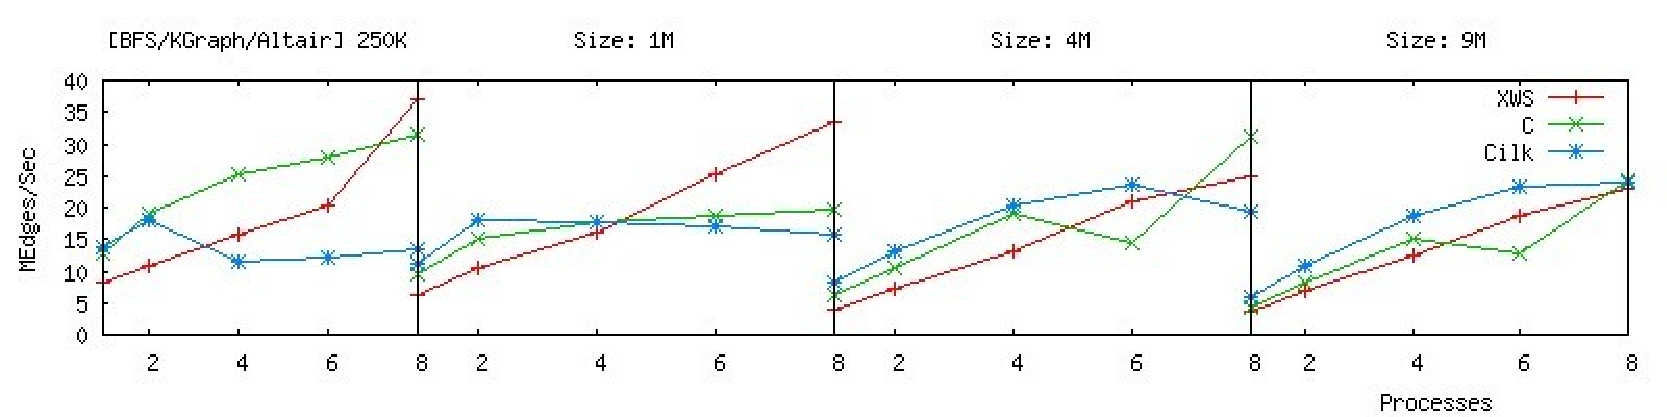
\includegraphics[width=10cm]{plots/bfs-kgraph-altair-color.pdf} \\
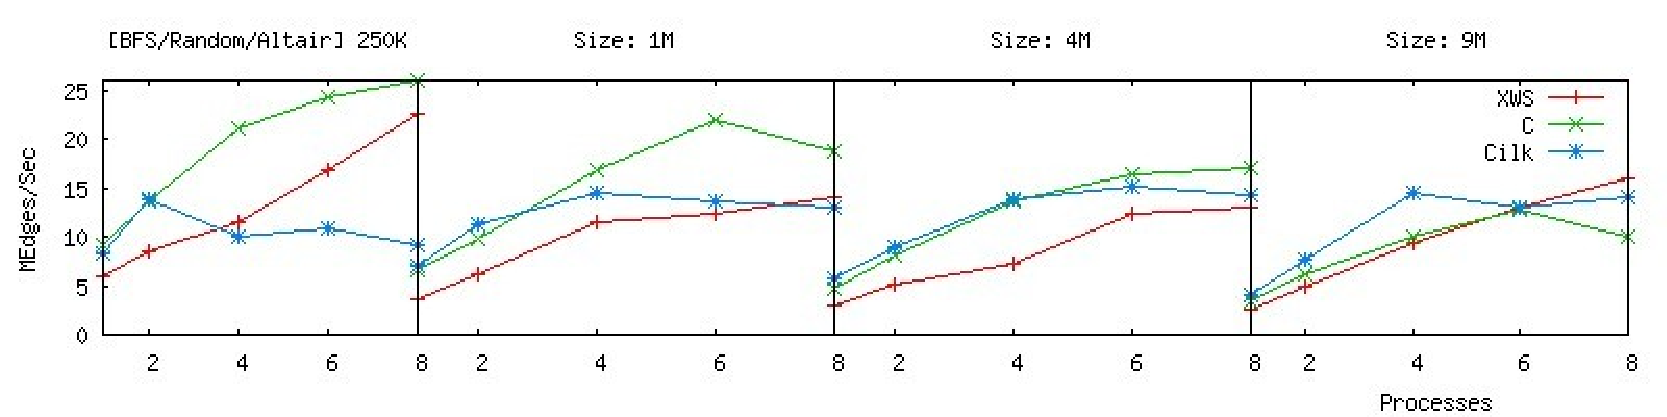
\includegraphics[width=10cm] {plots/bfs-random-altair-color.pdf} \\
\end{tabular}
\caption{BFS for Opteron}\label{altair}
\end{center}
\end{figure*}

\begin{figure*}
\begin{center}
 \begin{tabular}{ccc}
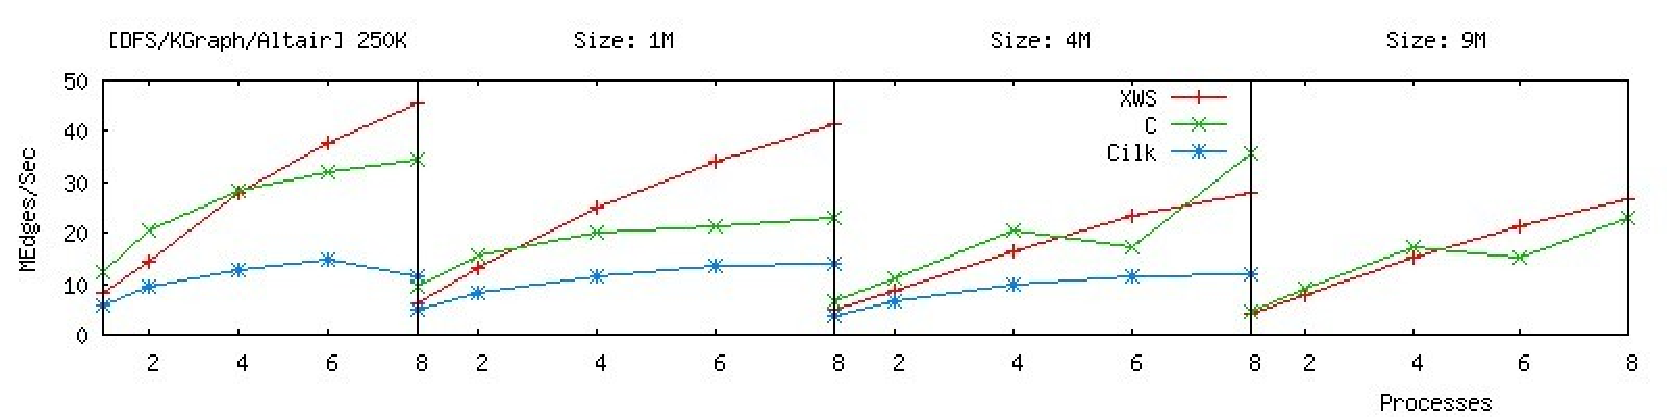
\includegraphics[width=10cm]{plots/dfs-kgraph-altair-color.pdf}\\
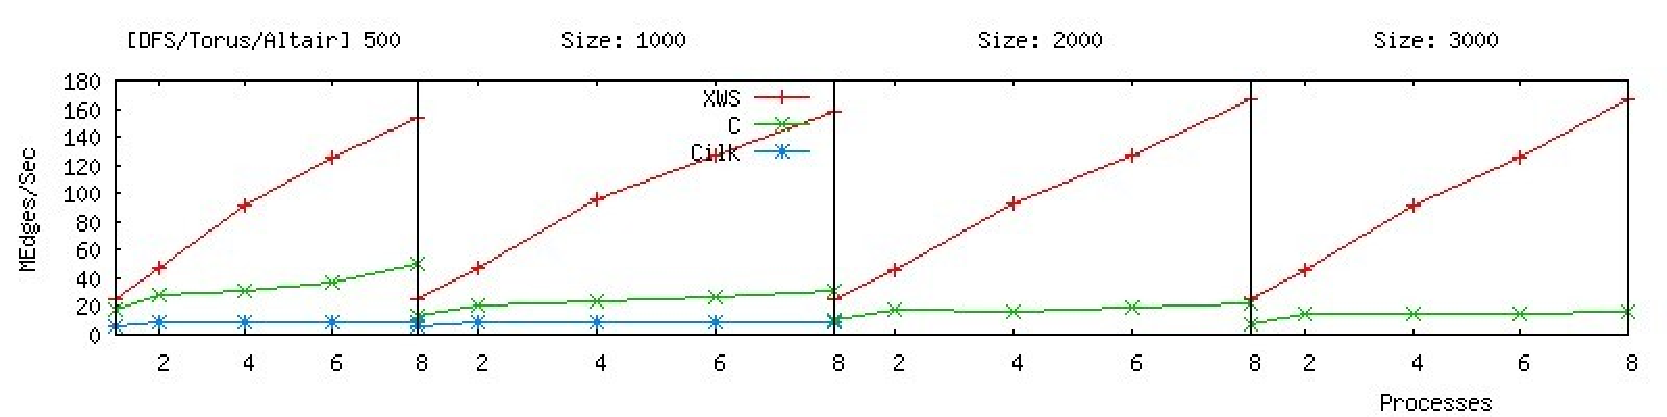
\includegraphics[width=10cm]{plots/dfs-torus-altair-color.pdf}\\
\end{tabular}
\caption{DFS for Opteron}\label{altair}
\end{center}
\end{figure*}

\begin{figure*}
\begin{center}
 \begin{tabular}{ccc}
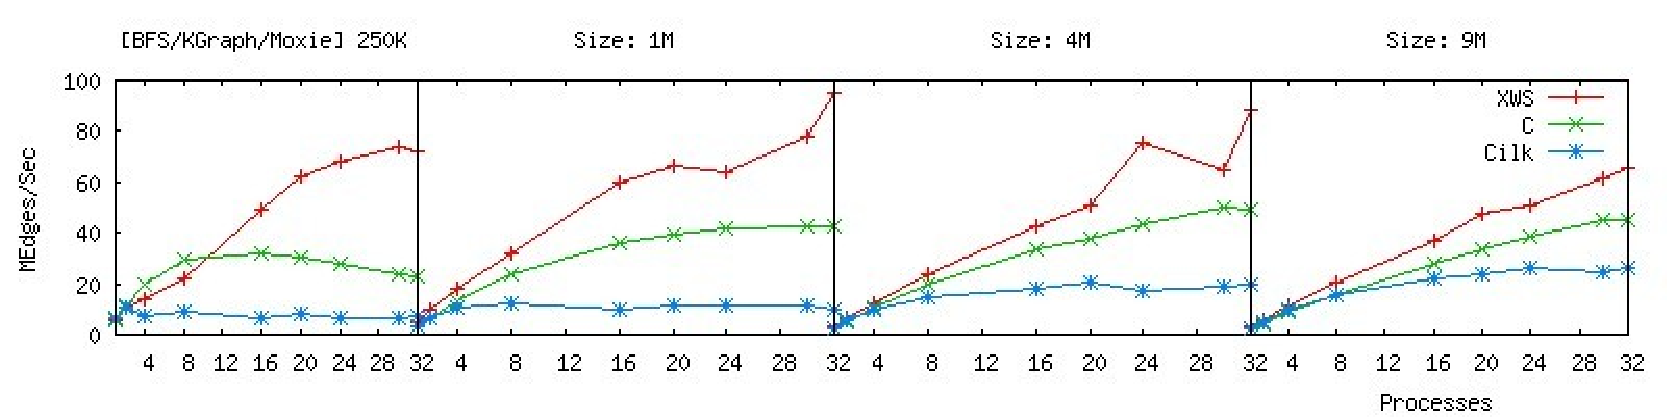
\includegraphics[width=10cm]{plots/bfs-kgraph-moxie-color.pdf} \\
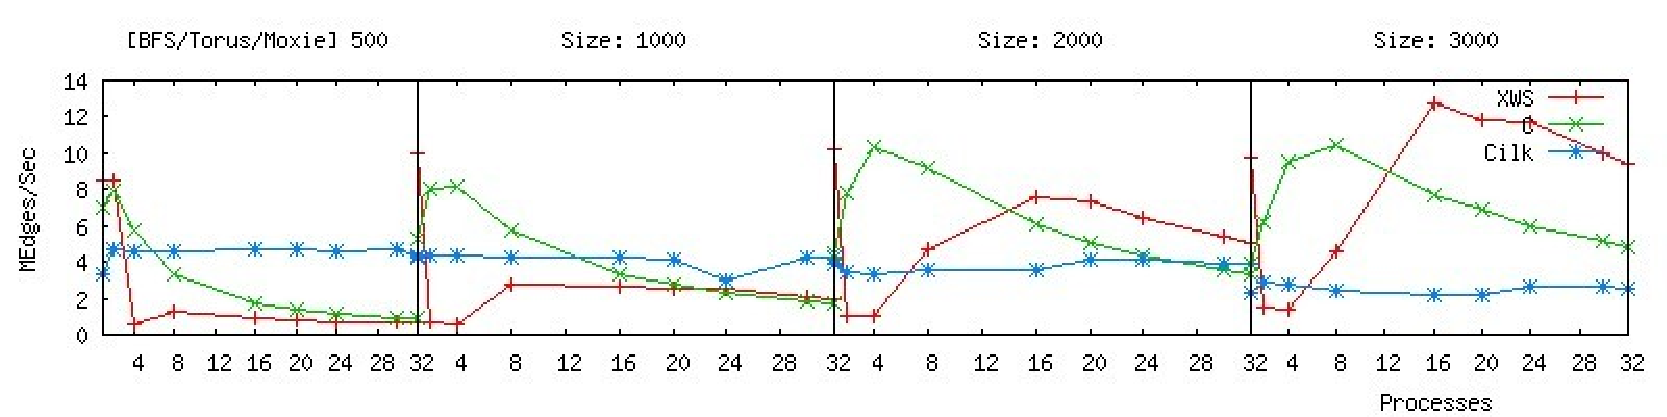
\includegraphics[width=10cm]{plots/bfs-torus-moxie-color.pdf} \\
 \end{tabular}
\caption{BFS for Niagara}\label{moxie-1}
\end{center}
\end{figure*}

\begin{figure*}
\begin{center}
 \begin{tabular}{ccc}
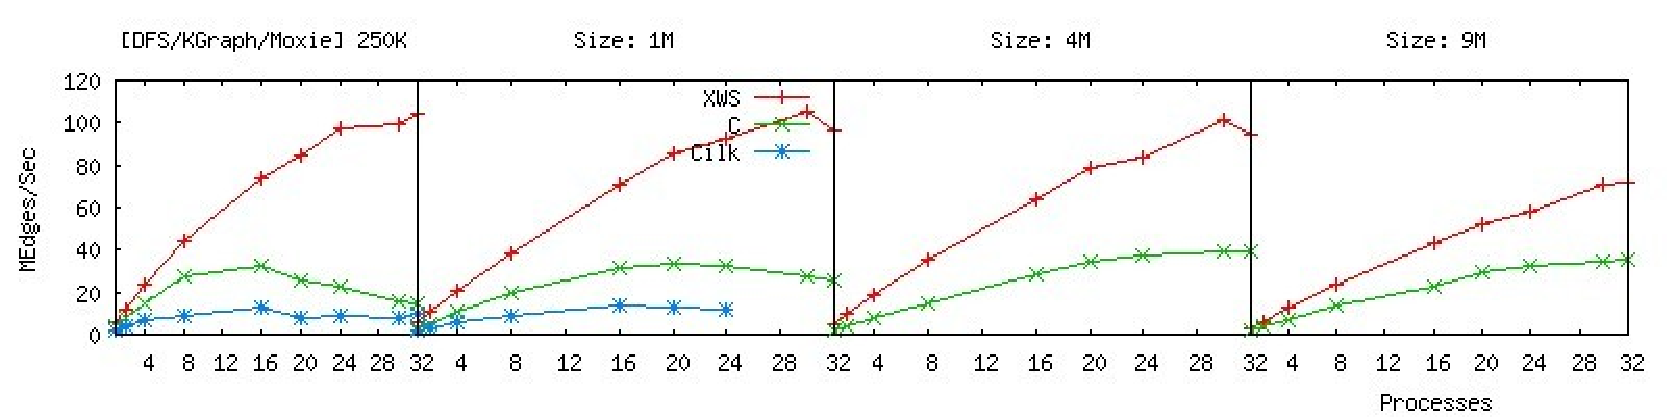
\includegraphics[width=10cm]{plots/dfs-kgraph-moxie-color.pdf}\\
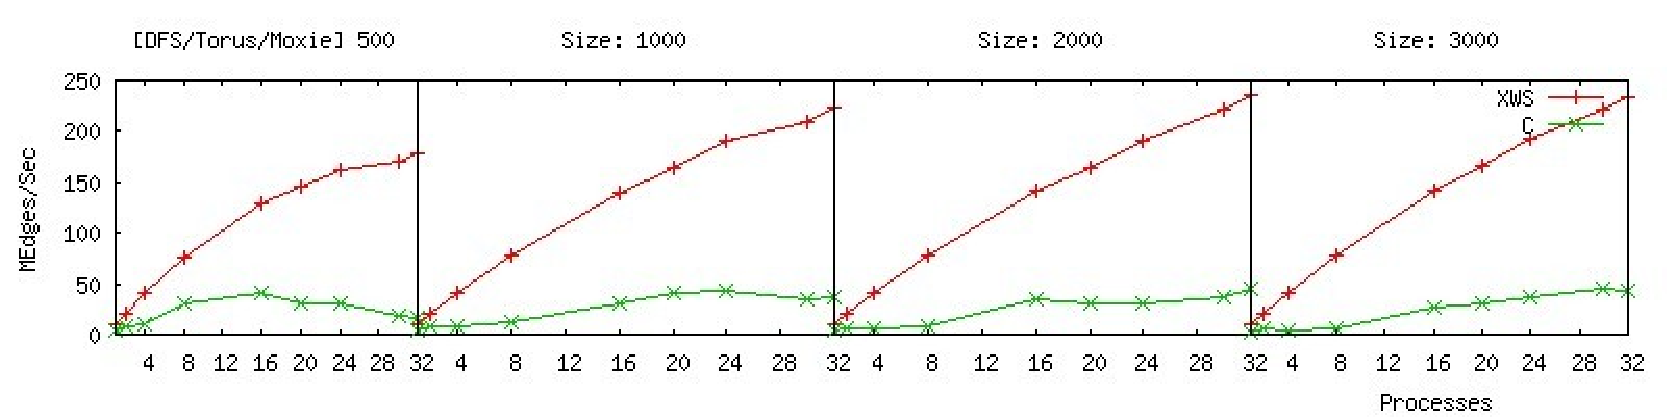
\includegraphics[width=10cm]{plots/dfs-torus-moxie-color.pdf}\\

 \end{tabular}
\caption{DFS for Niagara}\label{moxie-2}
\end{center}
\end{figure*}

\subsection{SIMPLE implementation (C)}

The C implementation of DFS works as follows. First a small stub-tree
of size $O(p^2)$ is generated by one thread randomly walking the graph
starting from the root.  The vertices encountered in the walk are
evenly distributed into the stacks of the $p$ threads. Each thread
then starts traversing the graph in DFS order.  To prevent race
conditions during DFS traversals, lock-free protocols are used to
guard against multiple threads coloring the same vertex. For
load-balancing, a thread attempts to steal a piece of the stack from
another thread in case it runs out of work. As a heuristic, each steal
takes one half of the stack from the victim. Note that in order to
reduce the cost of stealing, no synchronization is invoked in such
steals. The steals may get stale values, yet the correctness is not
jeopardized as the thread will later find all the stolen vertices have
been visited.  When all threads run out of work and there is no work
to steal, the algorithm halt. The stacks and their top and bottom
pointers are declared as volatile, and each push/pop operation
involves operations on volatiles.

The C implementation of parallel BFS follows the SPMD programming
paradigm. The expansion of the BFS frontier is implemented as
follows. Each thread keeps a local queue, and gets an equal portion of
vertices in the current frontier. In the beginning, there is only one
vertex (root) in the frontier, and only one thread has an non-empty
local queue. After draining the current frontier vertices in the
queue, new frontier vertices are placed inside the queue. When all
threads are done with the current frontier (guaranteed with a
barrier), the newly-added vertices in the queues are merged together
to form the new global frontier. Repetitive appearances of nodes in
the frontier is allowed. The algorithm iterates until no new frontier
vertices are discovered.

\subsection{Cilk implementation}

The Cilk implementation of parallel DFS can be derived easily from the
sequential recursive DFS. Instead of sequential traversal, we spawn a
parallel DFS traversal for each unvisited child of the
current vertex. To guard against race conditions among traversals, the
access to the color of a vertex is protected by lock-free
synchronizations. Load-balancing is handled by the Cilk runtime
library. However, as discussed earlier Cilk forces each procedure to
wait for termination of all its children spawned during its execution.

In the sequential implementation of BFS, iteration is over the vertices in the current frontier. Their unvisited neighbors are then used to form the next frontier. To achieve scalability in Cilk, the iteration has to be performed in a divide-and-conquer recursive way so as to utilize the Cilk work-stealing scheduler. The current frontier is partitioned into blocks and the base case in the recursion is the iteration over a single block. As in
the C implementation, repetitive appearances of vertices in a frontier is
allowed. The algorithm iterates until the next frontier is empty.


\subsection{\XWS{} implementation}\label{sec:Performance}

The core code for the \XWS{} implementations is presented in 
Section~\ref{sec:intro}.  We now discuss batching.


%%While classic graph traversals such as DFS and BFS can be supported by
%%XWS, they do not take advantage of some of the algorithm design
%%techniques that exploit work-stealing to provide performance superior
%%to that of other approaches to parallel programming.
%%
%%Work-stealing schemes are natural fits for many classic parallel
%%divide-and-conquer algorithms. (In fact, for some problems and
%%criteria, work-stealing provides optimizal solutions.) For example, to
%%process all of the elements of an array $A$ of size $N$, a root task
%%represents {$A$, $0$, $N$} which is then subdivided into two tasks
%%{$A$, $0$, $n/2$} and {$A$, $n/2$, $n$}, and so on until the size of each
%%task is less than an empirically-guided sequential threshold
%%indicating that further subdivision is not profitable because the task
%%overhead would be greater than the amount of work to process the task
%%sequentially. Notice that in a shared memory environment, the memory
%%needed for task descriptions themselves is small and constant.
%%
Algorithms for irregular graph problems are in general not directly
amenable to divide-and-conquer recursive decomposition. However, we
can still approximate the properties that make work-stealing perform
well for these problems.

To do this, we first require compact task descriptions.  The size of a
task description representing exploration starting at each of $k$ nodes
should be constant, and independent of $k$. Otherwise, the communication
overhead of pushing and stealing nodes would overwhelm processing,
especially in algorithms such as spanning trees, where the per-node
costs merely amount to marking nodes and labelling their parents.  We
address this by building up lists of work via simple linking: Each
node enqueued in the work-stealing queue is the head of a singly
linked list possibly containing other nodes as well. The ordering of
this list matters only in terms of memory locality and interference
with other threads, which favors simple stack-based linking.

We next ask, what value of $k$ should be used to batch a set of
unprocessed nodes. For any given node in an arbitrary graph, we cannot
know the value that will maximize aggregate throughput.
One choice is to empirically choose some fixed value. However,
the use of any fixed value would be too large during start up
(stalling all but the initial thread), and/or too small during
steady state. We can do better by first characterizing the
best values to use at boundary points:
\begin{itemize}
  \item A queued root node represents all of the work in the graph, so
    requires $k=1$.
  \item If processing has nearly completed, and all remaining nodes are
    dead-ends (i.e., leading to no further expansion) choosing the
    best value of $k$ is the counterpart to choosing the sequential
    threshold of a divide-and-conquer algorithm.  This value, $S$, is an
    empirical threshold relating algorithmic work versus framework
    overhead.  
\end{itemize}

Unless the per-node costs of an application are high enough to dictate
that $S=1$ (which is not the case for spanning tree algorithms), a rule
that causes $k$ to vary from $1$ at roots to $S$ at collections of dead-ends
will provide better load balance and throughput than one that would use a
fixed value. For some special graph types, it is possible to determine
a fixed function of this form. For example, if the graph were actually
a balanced tree, $k$ should increase exponentially from the root to the
leaves. However, in an arbitrary graph, any approach based on distance
from roots would be prone to arbitrarily poor estimates.  Instead, each
task may use its current work-stealing queue depth to help estimate
global progress properties: If the queue is empty, then even a single
node placed on it is potentially valuable to some other thread trying
to steal it and further expand.  Conversely, if the queue is very
large, then other threads must be busy processing other nodes, and any
newly discovered node is less likely to lead to further expansion.
Using a simple bounded exponential growth function (here, powers of
two) across these points maintains scaling properties: Each of the 
$2^j$ nodes in a batch of a size-$j$ queue (for $j \leq log_2(S)$) should have
$2^{-j}$ of the expected expansions as does the single node in a size $1$
queue. The choice of base two exponents is not entirely forced here,
and different constants might be better for some graph types.
However, the choice does coincide with the scaling and throughput
properties of work-stealing in the case of divide-and-conquer over
balanced binary trees, and adaptively approximates this case by
dynamically varying batch sizes based on differential steal rates.

The resulting basic algorithm is a simple variant of the DFS algorithm
presented in Section \ref{s:intr}: Each task accepts a list headed by one of its
nodes.  For each node, it labels and expands the edges into a new
list, pushing that list onto work-stealing queue when its size
exceeds $min(2^{Q}, S)$, where $Q$ is the queue-size. Notice that in
the case of $S=1$ (which might be used for algorithms with high
per-node processing costs), this is identical to plain DFS.

Our adaptive DFS improves on the implementation of this idea by
incorporating another common work-stealing programming technique. In
classic divide-and-conquer programs, co-execution of two tasks $a$ and $b$
is best implemented by forking $a$, then directly running $b$, and then
joining $a$.  This saves the overhead of pushing and then immediately
popping and running $b$.  We adapt this idea here via some bookkeeping
to swap lists rather than pushing and then immediately popping a new
list when the original list is exhausted. The performance improvements
stemming from this technique are always worthwhile, because they
decrease overhead without changing any other algorithmic
properties. However, as shown below, the extent of the improvement may
vary dramatically across different graph topologies.

As is the case with any work-stealing algorithm, the value of $S$ must
be empirically derived. Thresholds are functions of per-node
application costs (here, marking and setting spanning tree parents),
as well as underlying per-task framework costs (mainly, work-stealing
queue operations), as well as platform-level costs (processor
communication, memory locality effects and  garbage collection), along
with interactions among these, and so resist simple analytic
derivation.  However, each of these component factors are properties
of the program, and not, in general, its inputs (i.e., the actual
graphs).  As is the case for all work-stealing algorithms, choosing
values of S larger than necessary will increase the variance of
expected throughput: In some executions this may actually increase
throughput due to less queue overhead, but in others, a too-large
value will cause load imbalances, decreasing throughput.  But
sensitivity curves across these values are shallow within broadly
acceptable ranges. We find that restricting values to powers of two
suffices.

\paragraph{Choice of Threshold}

This choice of threshold was empirically guided by comparing
performance across powers of two. The impact of this choice varies
across graph types. Normalizing to $1.0$ for $S$ of $128$,
Table~\ref{table:rel-perf} shows throughput differences for graphs of
$4$ million nodes.  The best value of $S$ indicates that \XWS{} framework
overhead is low enough so that it is profitable to parallelize even batches
of only a $100$ or so dead-end nodes. The drop-off beyond $128$ is
very shallow, so larger values could have been used with almost no
loss.  However, choosing thresholds nearer the lower range of
estimated maxima reduces run-to-run variability.

\begin{table}
{\footnotesize
\begin{verbatim}
          Niagara             Opteron
S       T     K   R       T      K    R
1      0.58 0.79 0.81    0.18  0.54  0.55
2      0.68 0.85 0.85    0 33  0.78  0.81
8      0.88 0.93 0.94    0.75  0.97  0.93
32     0.97 1.00 0.99    0.82  0.98  0.94
128    1.00 1.00 1.00    1.00  1.00  1.00
512    0.98 0.92 1.00    0.89  1.00  0.99
2048   0.96 0.92 0.91    0.86  0.97  0.97
\end{verbatim}}
\caption{Relative performance across thresholds}\label{table:rel-perf}
\end{table}
While adaptive batching improves performance over DFS (equivalent to
$S=1$) across graph types, the extent of the improvement varies
considerably across graph types. This is due to two main factors,
{\em locality} and {\em connectivity}.

\paragraph{Locality} The graphs used in these experiments are too large to fit
into processor caches. Thus, cache misses have a huge impact on
performance. The Torus graph is laid out such that each node's
row-wise neighbors will normally be adjacent to it in memory, and
column-wise neighbors a constant stride away. Thus, traversals of a
torus that improve search locality will improve throughput.  This
effect can be quantified by comparing the performance of simply
accessing all of the nodes of the graph via all of its edges in some
predefined locality-sensitive versus locality-insensitive order.  As a
demonstration, the table below shows the relative
improvement of a full scan of each edge of each node when performed in
stride-1 index order of nodes versus a (wrapped around) stride of
$7919$ -- chosen as a prime large enough to minimize cache hits.  
\begin{table}
{\footnotesize
\begin{verbatim}
        opteron niagara
T       7.4     2.2
K       1.3     1.2
R       1.4     1.2
\end{verbatim}}
\caption{Locality effects across different graph types and platforms}
\end{table}
The
effects on the (4 dual) Opteron, especially for the Torus graph, are
much larger than on the (single multicore) Niagara. This is due to the
higher relative value of hardware prefetching across processors on the
Opteron when locality prevails.  These results independently indicate
that the ability of adaptive batching to better preserve locality of
access can be either a major or minor source of improvement, depending
on graph layout.  And for torus graphs, spanning tree construction
throughput exceeds that of simple locality-insensitive traversal.

\paragraph{Connectivity}  For densely or regularly connected graphs, the
ability of a task to swap in a partially created batch when its
initial batch is exhausted increases the actual nodes processed per
task, up from its nominal value of less than $S$, to the average number
of nodes that may be traversed, with backup partial buffer size of at
most $S$, before hitting a dead end. This value varies significantly
across the three graph types we have investigated. For $S=128$, the
average values on the Niagara ranges from $150$ for random graph, to $270$
for k-graphs, to $2400$ for Torus. (Opteron results are similar.) As the
number of nodes per task increases, so does throughput: Bypassing the
work-stealing queue reduces per-node overhead.  Lower queue access
rates in turn lead to lower contention for threads attempting to steal
work. While these effects are secondary to others described above,
they appear to account for the remaining throughput differences across
graph types.

%\subsubsection{Adaptive BFS}

Construction of adaptive BFS in the style of our adaptive DFS
encounters some new obstacles.  BFS proceeds in phases; batching
decisions must apply to next phase, not the current phase. Thus,
decisions cannot rely on current queue state.  Instead we employ a
predictive strategy to control batch sizes. During each phase, each
thread uses its estimate of average workload in the previous phase to
control batch size. Although other choices are possible, we used for
the experiments in Figure~\ref{altair},\ref{moxie}, constant multiples of
the previous estimate, bounded by minimum and maximum sizes. This
requires the multiplier to use as an empirically guided tuning
parameter.

The results demonstrate improvement over non-adaptive versions,
although less extreme than DFS.  We believe that the differences in
magnitude of effects are mainly due to three factors. First, because
BFS requires phased computation, improvements are limited by
underlying barrier synchronization rates (e.g.{} the Opteron's hardware
prefetching does not come into play). Second, our batch size
estimation strategy for BFS cannot be as sensitive to transient
dynamic imbalances as DFS.  And third, the BFS version does not enjoy
as many of the added locality benefits of DFS in-place list-swapping.
As further evidence of this third effect, the best tuning threshold
was higher, and showed sharper sensitivity, on the Opteron MP than the
Niagara multicore, which matches the locality and caching patterns
discussed above.

We leave for future work the investigation of other adaptive rules which may yield better performance. 


\subsection{Results}



We present results in Figure~\ref{altair} for runs of BFS (KGraph,
Random) and DFS (Kgraph, Torus) on Opteron and in Figure~\ref{moxie}
for runs of BFS (KGraph,Torus) and DFS (KGraph, Torus) on Niagara
(y-axis: MEPS, x-axis: P), for 250K, 1M, 4M and 9M vertices.  (Note
that the number of vertices in a torus is the square of the torus
size.) We see that on Opteron \XWS{} code is comparable with Cilk and
C code for BFS (Torus not shown), but substantially outperforms them
for DFS. On Niagara, \XWS{} code substantially outperforms Cilk and C
for all three graphs.\footnote{Several Cilk runs did not complete
successfully and are hence omitted.}


%\input runtime
%\input perf-eval
\input conclusion
{\footnotesize
\bibliographystyle{ieee}
\bibliography{paper,parallel,main-new}
}


\end{document}

